% answers.tex —— 2003 年·全国新课程卷·理科 · 参考答案与详细解析片段
% 由 tools/generate_projects.py 依来源总账自 2003/2003_数学真题_全国新课程理_试题.md + 2003/2003_数学真题_全国新课程理_解析正文.md + 2003/2003_数学真题_全国新课程理_答案要点.md 生成，勿手改（改源 MD 后重跑）


\begin{gktip}
固定源 PDF 为印刷页码 142–143 的两页题面，不附答案。以下解析均依据固定源独立复算；第 15、16、17、18 题图形在 LaTeX 工程中以 TikZ/PGFPlots 矢量源重绘。
\end{gktip}

\gkpart{一、选择题}

\begin{answer}
\gksolhead{1}{}

\textbf{题目}：

\Needspace{5\baselineskip}
复数

\nopagebreak[4]
\[
\frac{1-\sqrt3 i}{(\sqrt3+i)^2}
\]

的值为\mbox{（　　）}

（A）$\dfrac14+\dfrac{\sqrt3}{4}i$　　（B）$-\dfrac14-\dfrac{\sqrt3}{4}i$

（C）$\dfrac12+\dfrac{\sqrt3}{2}i$　　（D）$-\dfrac12-\dfrac{\sqrt3}{2}i$

\Needspace{4\baselineskip}
\textbf{解析}

\Needspace{5\baselineskip}
直接有

\nopagebreak[4]
\[
\frac{1-\sqrt3i}{(\sqrt3+i)^2}
=-\frac14-\frac{\sqrt3}{4}i,
\]

选 B。

\gkanswer{答案：B}

\end{answer}
\begin{answer}
\gksolhead{2}{}

\textbf{题目}：

已知 $x\in\left(-\dfrac\pi2,0\right)$，$\cos x=\dfrac45$，则 $\tan2x=$\mbox{（　　）}

（A）$\dfrac7{24}$　　（B）$-\dfrac7{24}$　　（C）$\dfrac{24}{7}$　　（D）$-\dfrac{24}{7}$

\Needspace{4\baselineskip}
\textbf{解析}

$\tan x=-3/4$，故 $\tan2x=-24/7$，选 D。

\gkanswer{答案：D}

\end{answer}
\begin{answer}
\gksolhead{3}{}

\textbf{题目}：

\Needspace{5\baselineskip}
设函数

\nopagebreak[4]
\[
f(x)=
\begin{cases}
2^{-x}-1,&x\leqslant0,\\
x^2,&x>0,
\end{cases}
\]

若 $f(x_0)>1$，则 $x_0$ 的取值范围是\mbox{（　　）}

（A）$(-1,1)$　　（B）$(-1,+\infty)$

（C）$(-\infty,-2)\cup(0,+\infty)$　　（D）$(-\infty,-1)\cup(1,+\infty)$

\Needspace{4\baselineskip}
\textbf{解析}

分段解 $f(x_0)>1$ 得 $x_0<-1$ 或 $x_0>1$，选 D。

\gkanswer{答案：D}

\end{answer}
\begin{answer}
\gksolhead{4}{}

\textbf{题目}：

\Needspace{5\baselineskip}
$O$ 是平面上一定点，$A\text{、}B\text{、}C$ 是平面上不共线的三个点，动点 $P$ 满足

\nopagebreak[4]
\[
\overrightarrow{OP}
=\overrightarrow{OA}
+\lambda\left(
\frac{\overrightarrow{AB}}{|\overrightarrow{AB}|}
+\frac{\overrightarrow{AC}}{|\overrightarrow{AC}|}
\right),\qquad \lambda\in[0,+\infty),
\]

则 $P$ 的轨迹一定通过 $\triangle ABC$ 的\mbox{（　　）}

（A）外心　　（B）内心　　（C）重心　　（D）垂心

\Needspace{4\baselineskip}
\textbf{解析}

\nopagebreak[4]
\[
\overrightarrow{AB}/|AB|+\overrightarrow{AC}/|AC|
\]

是角 $A$ 的内角平分线方向，轨迹从 $A$ 出发并通过内心，选 B。

\gkanswer{答案：B}

\end{answer}
\begin{answer}
\gksolhead{5}{}

\textbf{题目}：

\Needspace{5\baselineskip}
函数

\nopagebreak[4]
\[
y=\ln\frac{x+1}{x-1},\qquad x\in(1,+\infty)
\]

的反函数为\mbox{（　　）}

（A）$y=\dfrac{e^x-1}{e^x+1},\ x\in(0,+\infty)$

（B）$y=\dfrac{e^x+1}{e^x-1},\ x\in(0,+\infty)$

（C）$y=\dfrac{e^x-1}{e^x+1},\ x\in(-\infty,0)$

（D）$y=\dfrac{e^x+1}{e^x-1},\ x\in(-\infty,0)$

\Needspace{4\baselineskip}
\textbf{解析}

\Needspace{5\baselineskip}
反解

\nopagebreak[4]
\[
e^y=\frac{x+1}{x-1}
\Longrightarrow x=\frac{e^y+1}{e^y-1}.
\]

交换变量并注意定义域，选 B。

\gkanswer{答案：B}

\end{answer}
\begin{answer}
\gksolhead{6}{}

\textbf{题目}：

棱长为 $a$ 的正方体中，连接相邻面的中心，以这些线段为棱的八面体的体积为\mbox{（　　）}

（A）$\dfrac{a^3}{3}$　　（B）$\dfrac{a^3}{4}$　　（C）$\dfrac{a^3}{6}$　　（D）$\dfrac{a^3}{12}$

\Needspace{4\baselineskip}
\textbf{解析}

正方体被相邻面中心连成的八面体分成 8 个全等四面体，每个体积为 $a^3/48$，总和为 $a^3/6$，选 C。

\gkanswer{答案：C}

\end{answer}
\begin{answer}
\gksolhead{7}{}

\textbf{题目}：

设 $a>0$，$f(x)=ax^2+bx+c$，曲线 $y=f(x)$ 在点 $P(x_0,f(x_0))$ 处切线的倾斜角的取值范围为 $\left[0,\dfrac\pi4\right]$，则 $P$ 到曲线 $y=f(x)$ 对称轴距离的取值范围为\mbox{（　　）}

（A）$\left[0,\dfrac1a\right]$　　（B）$\left[0,\dfrac1{2a}\right]$

（C）$\left[0,\dfrac{|b|}{2a}\right]$　　（D）$\left[0,\dfrac{|b-1|}{2a}\right]$

\Needspace{4\baselineskip}
\textbf{解析}

\Needspace{5\baselineskip}
切线斜率 $2ax_0+b\in[0,1]$，点到对称轴的距离为

\nopagebreak[4]
\[
\frac{|2ax_0+b|}{2a}\in\left[0,\frac1{2a}\right],
\]

选 B。

\gkanswer{答案：B}

\end{answer}
\begin{answer}
\gksolhead{8}{}

\textbf{题目}：

\Needspace{5\baselineskip}
已知方程

\nopagebreak[4]
\[
(x^2-2x+m)(x^2-2x+n)=0
\]

的四个根组成一个首项为 $\dfrac14$ 的等差数列，则 $|m-n|=$\mbox{（　　）}

（A）$1$　　（B）$\dfrac34$　　（C）$\dfrac12$　　（D）$\dfrac38$

\Needspace{4\baselineskip}
\textbf{解析}

将四根写成首项 $1/4$ 的等差数列并代入两个二次因式的韦达关系，得 $|m-n|=1/2$，选 C。

\gkanswer{答案：C}

\end{answer}
\begin{answer}
\gksolhead{9}{}

\textbf{题目}：

已知双曲线中心在原点且一个焦点为 $F(\sqrt7,0)$，直线 $y=x-1$ 与其相交于 $M\text{、}N$ 两点，$MN$ 中点的横坐标为 $-\dfrac23$，则此双曲线的方程是\mbox{（　　）}

（A）$\dfrac{x^2}{3}-\dfrac{y^2}{4}=1$　　（B）$\dfrac{x^2}{4}-\dfrac{y^2}{3}=1$

（C）$\dfrac{x^2}{5}-\dfrac{y^2}{2}=1$　　（D）$\dfrac{x^2}{2}-\dfrac{y^2}{5}=1$

\Needspace{4\baselineskip}
\textbf{解析}

\Needspace{5\baselineskip}
代入直线并利用交点横坐标和，解得

\nopagebreak[4]
\[
\frac{x^2}{2}-\frac{y^2}{5}=1,
\]

选 D。

\gkanswer{答案：D}

\end{answer}
\begin{answer}
\gksolhead{10}{}

\textbf{题目}：

已知长方形的四个顶点 $A(0,0)\text{、}B(2,0)\text{、}C(2,1)\text{、}D(0,1)$，一质点从 $AB$ 的中点 $P_0$ 沿与 $AB$ 的夹角为 $\theta$ 的方向射到 $BC$ 上的点 $P_1$ 后，依次反射到 $CD\text{、}DA$ 和 $AB$ 上的点 $P_2\text{、}P_3$ 和 $P_4$（入射角等于反射角）。设 $P_4$ 的坐标为 $(x_4,0)$，若 $1<x_4<2$，则 $\tan\theta$ 的取值范围是\mbox{（　　）}

（A）$\left(\dfrac13,1\right)$　　（B）$\left(\dfrac13,\dfrac23\right)$　　（C）$\left(\dfrac25,\dfrac12\right)$　　（D）$\left(\dfrac25,\dfrac23\right)$

\Needspace{4\baselineskip}
\textbf{解析}

\Needspace{5\baselineskip}
矩形边界展开后，反射路径成为直线，由 $1<x_4<2$ 得

\nopagebreak[4]
\[
\frac25<\tan\theta<\frac12,
\]

选 C。

\gkanswer{答案：C}

\end{answer}
\begin{answer}
\gksolhead{11}{}

\Needspace{5\baselineskip}
\textbf{题目}：

\nopagebreak[4]
\[
\lim_{n\to\infty}
\frac{C_2^2+C_3^2+C_4^2+\cdots+C_n^2}
n(C_2^1+C_3^1+C_4^1+\cdots+C_n^1)
\]

的值为\mbox{（　　）}

（A）$3$　　（B）$\dfrac13$　　（C）$\dfrac16$　　（D）$6$

\Needspace{4\baselineskip}
\textbf{解析}

\Needspace{5\baselineskip}
用组合数求和公式化简（分母从 $C_2^1$ 开始）：

\nopagebreak[4]
\[
\frac{C_{n+1}^3}{n(C_{n+1}^2-1)}
\longrightarrow\frac13.
\]

选 B。

\gkanswer{答案：B}

\end{answer}
\begin{answer}
\gksolhead{12}{}

\textbf{题目}：

一个四面体的所有棱长都为 $\sqrt2$，四个顶点在同一球面上，则此球的表面积为\mbox{（　　）}

（A）$3\pi$　　（B）$4\pi$　　（C）$3\sqrt3\pi$　　（D）$6\pi$

\Needspace{4\baselineskip}
\textbf{解析}

棱长为 $\sqrt2$ 的正四面体外接球半径为 $\sqrt3/2$，球面面积为 $3\pi$，选 A。

\gkanswer{答案：A}

\end{answer}
\gkpart{二、填空题}

\begin{answer}
\gksolhead{13}{}

\textbf{题目}：

$\left(x^2-\dfrac1{2x}\right)^9$ 的展开式中 $x^9$ 的系数是\gkblank{}。

\Needspace{4\baselineskip}
\textbf{解析}

幂次条件 $18-3k=9$ 得 $k=3$，系数为 $-21/2$。

\gkanswer{答案：$-\dfrac{21}{2}$}

\end{answer}
\begin{answer}
\gksolhead{14}{}

\textbf{题目}：

某公司生产三种型号的轿车，产量分别为 1200 辆、6000 辆和 2000 辆。为检验该公司的产品质量，现用分层抽样的方法抽取 46 辆进行检验，这三种型号的轿车依次应抽取\gkblank{}、\gkblank{}、\gkblank{}辆。

\Needspace{4\baselineskip}
\textbf{解析}

抽样率为 $46/(1200+6000+2000)=1/200$，三层样本数为 $6\text{、}30\text{、}10$。

\gkanswer{答案：$6,30,10$}

\end{answer}
\begin{answer}
\gksolhead{15}{}

\textbf{题目}：

某城市在中心广场建造一个花圃，花圃分为 6 个部分（如图）。现要栽种 4 种不同颜色的花，每部分栽种一种且相邻部分不能栽种同样颜色，不同的栽种方法有\gkblank{}种。（以数字作答）
\nopagebreak[4]
\begin{center}% 2003 年全国新课程理科第 15 题：花圃着色图
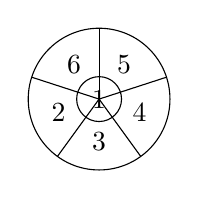
\begin{tikzpicture}[scale=0.75]
  \draw (0,0) circle (1.2);
  \foreach \angle in {90,18,-54,-126,162}
    \draw (0,0)--(\angle:1.2);
  \draw (0,0) circle (0.38);
  \node at (0,0) {1};
  \node at (54:0.72) {5};
  \node at (-18:0.72) {4};
  \node at (-90:0.72) {3};
  \node at (-162:0.72) {2};
  \node at (126:0.72) {6};
\end{tikzpicture}
\end{center}
\nopagebreak[4]
\Needspace{4\baselineskip}
\textbf{解析}

\Needspace{5\baselineskip}
中心区域有 $4$ 种选色，外围五个区域构成五边形环，剩余三色的合法着色数为

\nopagebreak[4]
\[
(3-1)^5-(3-1)=30.
\]

总数为 $4\times30=120$。

\gkanswer{答案：$120$}

\end{answer}
\begin{answer}
\gksolhead{16}{}

\textbf{题目}：

下列 5 个正方体图形中，$l$ 是正方体的一条对角线，点 $M\text{、}N\text{、}P$ 分别为其所在棱的中点，能得出 $l\perp$ 面 $MNP$ 的图形的序号是\gkblank{}。（写出所有符合要求的图形序号）
\nopagebreak[4]
\begin{center}% 2003 年全国新课程理科第 16 题：正方体选项示意
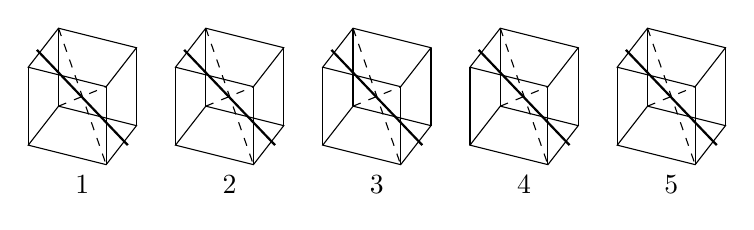
\begin{tikzpicture}[>=stealth,scale=0.55]
  \foreach \sx/\lab in {0/1,3.4/2,6.8/3,10.2/4,13.6/5}
  {
    \begin{scope}[shift={(\sx,0)}]
      \draw (0,0)--(1.8,-0.45)--(2.5,0.45)--(0.7,0.9)--cycle;
      \draw (0,0)--(0,1.8) (1.8,-0.45)--(1.8,1.35)
        (2.5,0.45)--(2.5,2.25) (0.7,0.9)--(0.7,2.7);
      \draw (0,1.8)--(1.8,1.35)--(2.5,2.25)--(0.7,2.7)--cycle;
      \draw[dashed] (0.7,0.9)--(1.8,1.35) (0.7,2.7)--(1.8,-0.45);
      \draw[thick] (0.2,2.2)--(2.3,0.0);
      \node at (1.25,-0.9) {\lab};
    \end{scope}
  }
\end{tikzpicture}
\end{center}
\nopagebreak[4]
\Needspace{4\baselineskip}
\textbf{解析}

逐图取坐标并检验对角线方向向量与面内两条独立向量的内积，符合垂直条件的图形为②、⑤。

\gkanswer{答案：②⑤}

\end{answer}
\gkpart{三、解答题}

\begin{answer}
\gksolhead{17}{}

\textbf{题目}：

\Needspace{5\baselineskip}
已知函数

\nopagebreak[4]
\[
f(x)=2\sin x(\sin x+\cos x).
\]

（1） 求函数 $f(x)$ 的最小正周期和最大值；

（2） 在给出的直角坐标系中，画出函数 $y=f(x)$ 在区间 $\left[-\dfrac\pi2,\dfrac\pi2\right]$ 上的图象。
\nopagebreak[4]
\begin{center}% 2003 年全国新课程理科第 17 题：函数图象坐标系
\begin{tikzpicture}[x=1.0cm,y=0.7cm,>=stealth]
  \draw[->] (-1.9,0)--(1.9,0) node[right] {$x$};
  \draw[->] (0,-1.4)--(0,1.6) node[above] {$y$};
  \node[below] at (-1.57,0) {$-\frac\pi2$};
  \node[below] at (1.57,0) {$\frac\pi2$};
  \node[below left] at (0,0) {$O$};
\end{tikzpicture}
\end{center}
\nopagebreak[4]
\Needspace{4\baselineskip}
\textbf{解析}

\gksubpart{(1)}

\nopagebreak[4]
\[
f(x)=1+\sqrt2\sin\left(2x-\frac\pi4\right).
\]

所以最小正周期为 $\pi$，最大值为 $1+\sqrt2$。在区间端点和零点处取值并平滑连接即可作图。

\gksubpart{(2)}

图象在题面给出的区间内按上述函数绘制。

\gkanswer{答案（1）：最小正周期为 $\pi$，最大值为 $1+\sqrt2$。}

\gkanswer{答案（2）：图象见解析版。}

\end{answer}
\begin{answer}
\gksolhead{18}{}

\textbf{题目}：

如图，在直三棱柱 $ABC-A_1B_1C_1$ 中，底面是等腰直角三角形，$\angle ACB=90^\circ$，侧棱 $AA_1=2$，$D\text{、}E$ 分别是 $CC_1$ 与 $A_1B$ 的中点，点 $E$ 在平面 $ABD$ 上的射影是 $\triangle ABD$ 的重心 $G$。
\nopagebreak[4]
\begin{center}% 2003 年全国新课程理科第 18 题：直三棱柱
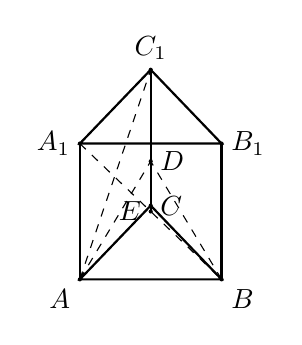
\begin{tikzpicture}[>=stealth,scale=0.75]
  \coordinate (A) at (0,0); \coordinate (B) at (2.4,0);
  \coordinate (C) at (1.2,1.25); \coordinate (A1) at (0,2.3);
  \coordinate (B1) at (2.4,2.3); \coordinate (C1) at (1.2,3.55);
  \coordinate (D) at (1.2,2.0); \coordinate (E) at (1.2,1.15);
  \draw[thick] (A)--(B)--(C)--cycle;
  \draw[thick] (A1)--(B1)--(C1)--cycle;
  \draw[thick] (A)--(A1) (B)--(B1) (C)--(C1);
  \draw[dashed] (A1)--(B) (A)--(C1) (A)--(D) (B)--(D);
  \draw[thick] (E)--(D);
  \fill (A) circle (1pt) node[below left] {$A$};
  \fill (B) circle (1pt) node[below right] {$B$};
  \fill (C) circle (1pt) node[right] {$C$};
  \fill (A1) circle (1pt) node[left] {$A_1$};
  \fill (B1) circle (1pt) node[right] {$B_1$};
  \fill (C1) circle (1pt) node[above] {$C_1$};
  \fill (D) circle (1pt) node[right] {$D$};
  \fill (E) circle (1pt) node[left] {$E$};
\end{tikzpicture}
\end{center}
\nopagebreak[4]
（1） 求 $A_1B$ 与平面 $ABD$ 所成角的大小（结果用反三角函数值表示）；

（2） 求点 $A_1$ 到平面 $AED$ 的距离。

\Needspace{4\baselineskip}
\textbf{解析}

\Needspace{5\baselineskip}
取

\nopagebreak[4]
\[
C=(0,0,0),\quad A=(2,0,0),\quad B=(0,2,0),
\]

\nopagebreak[4]
\[
C_1=(0,0,2),\quad A_1=(2,0,2),\quad B_1=(0,2,2).
\]

由投影条件可得底面直角边长为 $2$，并有 $D=(0,0,1)$、$E=(1,1,1)$。

\gksubpart{(1)}

\Needspace{5\baselineskip}
平面 $ABD$ 法向量为 $(1,1,2)$，$\overrightarrow{A_1B}=(-2,2,-2)$，故

\nopagebreak[4]
\[
\sin\alpha=\frac{|(-2,2,-2)\cdot(1,1,2)|}{\sqrt{12}\sqrt6}
=\frac{\sqrt2}{3}.
\]

所以 $\alpha=\arcsin(\sqrt2/3)$。

\gksubpart{(2)}

\Needspace{5\baselineskip}
平面 $AED$ 方程为 $x-y+2z-2=0$，因此

\nopagebreak[4]
\[
d(A_1,\text{\text{平面} }AED)=\frac4{\sqrt6}=\frac{2\sqrt6}{3}.
\]

\gkanswer{答案（1）：$\arcsin\dfrac{\sqrt2}{3}$}

\gkanswer{答案（2）：$\dfrac{2\sqrt6}{3}$}

\end{answer}
\begin{answer}
\gksolhead{19}{}

\textbf{题目}：

\Needspace{5\baselineskip}
设 $a>0$，求函数

\nopagebreak[4]
\[
f(x)=\sqrt{x}-\ln(x+a),\qquad x\in(0,+\infty)
\]

的单调区间。

\Needspace{4\baselineskip}
\textbf{解析}

\nopagebreak[4]
\[
f'(x)=\frac1{2\sqrt x}-\frac1{x+a}
=\frac{x-2\sqrt x+a}{2\sqrt x(x+a)}.
\]

\Needspace{5\baselineskip}
令 $t=\sqrt x$，分子为 $(t-1)^2+a-1$。若 $a\geqslant1$，函数在 $(0,+\infty)$ 上单调递增；若 $0<a<1$，令

\nopagebreak[4]
\[
\alpha=(1-\sqrt{1-a})^2,\qquad
\beta=(1+\sqrt{1-a})^2,
\]

则在 $(0,\alpha)$、$(\beta,+\infty)$ 上递增，在 $(\alpha,\beta)$ 上递减。

\gkanswer{答案：在 $0<a<1$ 时按 $(1\pm\sqrt{1-a})^2$ 分段单调；$a\geqslant1$ 时在 $(0,+\infty)$ 上单调递增。}

\end{answer}
\begin{answer}
\gksolhead{20}{}

\textbf{题目}：

$A\text{、}B$ 两个代表队进行乒乓球对抗赛，每队三名队员，$A$ 队队员是 $A_1\text{、}A_2\text{、}A_3$，$B$ 队队员是 $B_1\text{、}B_2\text{、}B_3$，按以往多次比赛的统计，对阵队员之间胜负概率如下：

\begin{center}
\begin{tabular}{lrr}
\toprule
对阵队员 & $A$ 队队员胜的概率 & $A$ 队队员负的概率 \\
\midrule
$A_1$ 对 $B_1$ & $\dfrac23$ & $\dfrac13$ \\
$A_2$ 对 $B_2$ & $\dfrac25$ & $\dfrac35$ \\
$A_3$ 对 $B_3$ & $\dfrac25$ & $\dfrac35$ \\
\bottomrule
\end{tabular}
\end{center}

现按表中对阵方式出场，每场胜队得 1 分，负队得 0 分，设 $A$ 队、$B$ 队最后所得总分分别为 $\xi\text{、}\eta$。

（1） 求 $\xi\text{、}\eta$ 的概率分布；

（2） 求 $E\xi\text{、}E\eta$。

\Needspace{4\baselineskip}
\textbf{解析}

\gksubpart{(1)}

\Needspace{5\baselineskip}
令 $\xi$ 为 A 队胜场数。三场独立，概率生成函数为

\nopagebreak[4]
\[
\left(\frac13+\frac23t\right)
\left(\frac35+\frac25t\right)^2.
\]

\Needspace{5\baselineskip}
故

\nopagebreak[4]
\[
P(\xi=0,1,2,3)
=\left(\frac3{25},\frac25,\frac{28}{75},\frac8{75}\right),
\qquad \eta=3-\xi.
\]

\Needspace{5\baselineskip}
期望为

\nopagebreak[4]
\[
E\xi=\frac{22}{15},\qquad E\eta=\frac{23}{15}.
\]

\gksubpart{(2)}

上式即为所求的两个数学期望。

\gkanswer{答案（1）：$\xi$ 的分布为 $\left(\dfrac3{25},\dfrac25,\dfrac{28}{75},\dfrac8{75}\right)$；$\eta=3-\xi$。}

\gkanswer{答案（2）：$E\xi=\dfrac{22}{15},\ E\eta=\dfrac{23}{15}$。}

\end{answer}
\begin{answer}
\gksolhead{21}{}

\textbf{题目}：

已知常数 $a>0$，向量 $\vec c=(0,a)$，$\vec i=(1,0)$。经过原点 $O$ 以 $\vec c+\lambda\vec i$ 为方向向量的直线与经过定点 $A(0,a)$ 以 $\vec i-2\lambda\vec c$ 为方向向量的直线相交于 $P$，其中 $\lambda\in\mathbb R$。试问：是否存在两个定点 $E\text{、}F$，使得 $|PE|+|PF|$ 为定值？若存在，求出 $E\text{、}F$ 的坐标；若不存在，说明理由。

\Needspace{4\baselineskip}
\textbf{解析}

\Needspace{5\baselineskip}
设交点参数为 $\lambda$，分别写两条直线的参数方程并消去参数，得到

\nopagebreak[4]
\[
2a^2x^2+y^2-ay=0,
\]

\Needspace{5\baselineskip}
即

\nopagebreak[4]
\[
2a^2x^2+\left(y-\frac a2\right)^2=\frac{a^2}{4}.
\]

\Needspace{5\baselineskip}
这是椭圆（临界值为圆）。当 $0<a<1/\sqrt2$ 时，焦点为

\nopagebreak[4]
\[
\left(\pm\frac12\sqrt{\frac12-a^2},\frac a2\right),
\qquad |PE|+|PF|=\frac1{\sqrt2};
\]

\Needspace{5\baselineskip}
当 $a>1/\sqrt2$ 时，焦点为

\nopagebreak[4]
\[
\left(0,\frac a2\pm\frac12\sqrt{a^2-\frac12}\right),
\qquad |PE|+|PF|=a.
\]

\gkanswer{答案：见解析版；轨迹为椭圆，焦点分类按 $a$ 与 $1/\sqrt2$ 的大小确定。}

\end{answer}
\begin{answer}
\gksolhead{22}{}

\textbf{题目}：

\Needspace{5\baselineskip}
设 $a_0$ 为常数，且

\nopagebreak[4]
\[
a_n=3^{n-1}-2a_{n-1},\qquad n\in\mathbb N^*.
\]

\Needspace{5\baselineskip}
（1） 证明对任意 $n\geqslant1$，

\nopagebreak[4]
\[
a_n=\frac15\left[3^n+(-1)^{n-1}\cdot2^n\right]+(-1)^n\cdot2^n a_0;
\]

（2） 假设对任意 $n\geqslant1$ 有 $a_n>a_{n-1}$，求 $a_0$ 的取值范围。

\Needspace{4\baselineskip}
\textbf{解析}

\gksubpart{(1)}

\Needspace{5\baselineskip}
由递推式 $a_2=4\text{、}a_3=13$。设

\nopagebreak[4]
\[
b_n=a_n-\frac15\left[3^n+(-1)^{n-1}2^n\right],
\]

\Needspace{5\baselineskip}
则 $b_n=-2b_{n-1}$，从而

\nopagebreak[4]
\[
a_n=\frac15\left[3^n+(-1)^{n-1}2^n\right]+(-1)^n2^na_0.
\]

\Needspace{5\baselineskip}
条件 $a_n>a_{n-1}$ 等价于 $a_{n-1}<3^{n-2}$。分别考察奇偶指标，并结合 $n=1$，得到

\nopagebreak[4]
\[
0<a_0<\frac13.
\]

\gksubpart{(2)}

这就是题设不等式条件下的参数范围。

\gkanswer{答案（1）：$a_2=4,\ a_3=13$；$a_n=\dfrac15[3^n+(-1)^{n-1}2^n]+(-1)^n2^na_0$。}

\gkanswer{答案（2）：$0<a_0<\dfrac13$。}

\end{answer}